\NeedsTeXFormat{LaTeX2e}
\documentclass[10pt,a4paper]{scrartcl}

\usepackage{tabularx,graphicx,setspace}

\ifx\pdfoutput\undefined
  % We're not running pdftex
  % european (better) fonts -- does not look good with pdflatex
  \usepackage[T1]{fontenc}
  \newcommand{\href}[2]{#2\\{\hspace*{5mm}\scriptsize <#1>}\\}
\else
  \pdfcompresslevel=9
  \def\pdfBorderAttrs{/Border [0 0 0] } % No border around Links
  \usepackage{hyperref}
\fi

\title{Project Equalizer}
\author{Stefan Eilemann\thanks{eilemann@gmail.com}\\[\medskipamount]
%  EyeScale Software Sarl
}
\date{\htmladdnormallink{http://www.equalizergraphics.com/}
  {http://www.equalizergraphics.com/}}

\newcommand{\tm}{\texttrademark~}
\newcommand{\rc}{\raise 1ex\hbox{{\tiny\textregistered}}~}
% suppress  single floating lines on top (widow) and bottom(club)
%  10000 is infinity
%  tradeoff: maybe underfull vboxes
\clubpenalty=10000
\widowpenalty=10000 

\oddsidemargin .5cm
\evensidemargin .5cm
\topmargin 1cm
\setlength{\textwidth}{15cm}
\setlength{\textheight}{20cm}
\begin{document}

% paragraph spacing -- should be rubber length
%\setlength{\parskip}{1.5ex plus 0.5ex minus 0.5ex}
% paragraph indention for the first line
%\setlength{\parindent}{0em}

\maketitle
\thispagestyle{empty}
% \begin{figure}[ht]
% \centering
% 
\includegraphics[width=5em]{logo.pdf}
% \end{figure}
\vfill
\abstract{
% what
Equalizer is a project to develop software to simplify the creation of scalable
graphics applications and to improve the usability of multipipe
visualization systems. The main components of Equalizer are a resource
server, which controls the visualization system's configuration, a
client side library for the development of scalable graphics software, a
transparent software layer to execute unmodified applications alongside
with scalable applications, as well as remote visualization
capabilities. Equalizer is designed to support all kinds of
visualization systems ranging from laptops, workstations, multipipe
shared memory systems to graphics clusters.

% why
The purpose of Equalizer is to build a foundation for high performance
visualization by providing a common base for all kinds of applications
used in multipipe environments, in particular for parallel graphics
software.

% how/when
The open development approach of Equalizer maximizes the benefits for
hardware vendors, software developers, research institutions and end
users. Interested parties are strongly encouraged to contact us. We are
looking for contributions or founding for several components of Equalizer.
}
\vfill
{\center\begin{tabularx}{.88\textwidth}{|l|l|X|}
\hline
\bf Version & \bf Date & \bf Changes \\
\hline
0.2         & October 5, 2006 & update status\\
0.1         & July 5, 2006    & initial draft\\
\hline
\multicolumn{3}{c}{\small Latest version at 
  \htmladdnormallink{http://www.equalizergraphics.com/documents/ProjectEqualizer.pdf}
  {http://www.equalizergraphics.com/documents/ProjectEqualizer.pdf}}\\
\end{tabularx}}
\clearpage
\pagenumbering{arabic}

\section{Overview}
As outlined in \cite{Analysis}, there are three fundamentally different
approaches to parallel rendering. Transparent solutions offer an easy
solution for applications which cannot or need not to be modified, but
are limited in performance and compatibility. Distributed
scene graphs offer better performance, but require the application
to use a certain scene graph. The third approach, a parallel rendering
framework offers a generic API for the development of parallel, scalable
graphics applications.

Today we have satisfying, though often proprietary, solutions for the
transparent approach\footnote{e.g., Chromium from Stanford University,
VGP from ModViz, SVN from IBM}. Distributed scene graphs are beginning
to emerge\footnote{e.g., ScaleViz from Mercury Computer Systems} as
well. There is currently no general programming framework to create
parallel graphics applications. Furthermore, all existing solutions are
'islands', that is, they are configured separately and do possibly
interfere with each other when running simultanously on the same
system. Equalizer addresses these issues.

Unlike the HPC community, visualization software developers do not
widely address performance bottlenecks by parallelizing
their applications. One of the reasons for the lack of parallel graphics
applications is the lack of a standard programming interface, which
implements specific knowledge needed to create scalable visualization
applications. Equalizer provides a programming framework for high
performance visualization.

\section{Project Description}

Equalizer is a project to create new software to facilitate the
development and usage of software for multipipe
graphics systems by addressing the shortcomings of the current
software situation. It adds the two missing components, a
parallel programming framework and a resource management system, and
integrates existing solutions, such as a transparent layer, scene graphs
and remote visualization capabilities.

Equalizer addresses all visualization systems. An Equalizer application
can run unmodified on a laptop, a multipipe workstation, a graphics
cluster or a multipipe shared memory visualization server.

\subsection{Development Model}

The Equalizer development is conducted in an open way. It is licensed
under the LGPL open source license. Contributing parties, such as
hardware vendors, software developers and end users, have the following
benefits from contributing to the project:

\begin{description}
\item[Lower Development Costs] The common functionality of any multipipe
  application is outsourced to the Equalizer framework, thus freeing the
  software developers to reimplement basic algorithms. The expertise for
  high performance visualization is partly embedded into Equalizer, and
  has not to be developed inhouse. The open development approach ensures
  that Equalizer delivers the functionality most needed by the community.
\item[Higher Functionality] Additional features, which would not be
  cost-effective to implement in the application, are provided by the
  Equalizer framework. New features will become available over time,
  and will often be usable by the application with no or minimal code
  changes.
\item[Ease of Use] The central resource management of Equalizer requires
  only a one-time setup, thus minimizing the impact for end users. Once
  a visualization system is set up, unmodified and scalable OpenGL
  applications can be run without any modification. Simple
  configurations, especially shared memory systems, will be configured
  automatically.
\item[Reduced Development Risk] The open source license of Equalizer is
  the guarantee for software developers that the product will be
  available indefinitely. Critical features or bugs, in case they are
  not addressed by the maintainers, can still be addressed internally.
\end{description}

\subsection{Programming Framework}

The programming framework is the main contribution of the
Equalizer project. It addresses common problems when creating parallel
graphics applications, and thus facilitates the development of scalable
multipipe rendering software. It addresses the process creation and
synchronization, rendering task distribution, data transport, and the
composition of the rendering results. The software developer plugs the
application's rendering code into the framework. The Equalizer server
deploys this rendering code according to the system's configuration and
load. The programming framework is the client library to the Equalizer
server, as well as the header files for this library.

\subsection{Resource Management System}

The core of the resource management system is the Equalizer server,
which is managing the system's configuration. It is configured to know the
system resources and schedules the execution of rendering tasks on these
resources. Equalizer applications provide a render client\footnote{The
  render client can be the same executable as the application.}, which
contains the application's rendering code. This render client is
instanciated on the render nodes by the Equalizer server. The
transparent layer and distributed scene graphs are technically an
Equalizer application. 

For standalone usage on simple machines, the Equalizer client library
will be able to automatically configure and use a builtin server, to
facilitate the deployment on workstations. Naturally, certain
optimisations, such as the per system loadbalancing is lost without the
use of a dedicated server.

\subsection{Integration}
The following components will be based on existing open source software, which
will be integrated with Equalizer. This integration enables a seamless
execution and end user experience. On one hand, by relying on the
Equalizer server for configuration, an visualization systems has only
one set of configuration files, instead of disjunct configurations for
each of the tools. On the other hand, the central resource management improves
the performance and interoperability between applications running on
the same system.

\subsubsection{Transparent Layer}
The transparent layer enables the execution of unmodified applications
on the cluster. Applications which do not run at the required
performance can then be addressed individually by porting them to
directly use the Equalizer programming framework. This transparent layer
will most likely be built using the Chromium\cite{Humphreys02}
framework. For usability reasons, a virtualization solution for the 2D
user interface, such as Xdmx X11 proxy server, will be integrated with
the Equalizer core and the transparent layer.

\subsubsection{Remote Visualization}
Remote visualization provides the capability of executing the
application on a powerful, central visualization system. The integration
with Equalizer allows for seamless integration of remote visualization,
and enables optimisations due to the knowledge gathered by the
framework during rendering.

\subsubsection{Scene Graphs}
The integration with scene graphs enables existing applications
using such a scene graph to quickly be able to take advantadge of
multipipe systems.

Two different approaches might be taken. In the first approach, each render node
holds a copy of the scene graph, and applies the changes made by the
application. In the second approach, the application sends high-level
rendering commands to the nodes, which together with a caching mechanism
can provide excellent performance.

\section{Milestones}

Much of the development of Equalizer is driven by the actual need of the
users, which are at the moment the software developers. 

Currently, the programming framework is usable for the development of
commercial multipipe applications by an experienced OpenGL
programmer. By the end of 2006, we will have implemented the core
scalable rendering engine to show the benefits of scalable rendering on
commodity graphics clusters.

The transparent layer will be developed in 2007. The founding for this
effort is currently investigated. Interested parties are strongly
encouraged to contact us with proposals.

\subsection{Programming Framework}
The core part of the Equalizer project is the programming framework and
resource server. Naturally, these two components are the first major
milestone. Currently, they are usable to start the development of
parallel graphics applications. Right now Equalizer supports multipipe
rendering for display walls and immersive virtual reality installations,
including stereo and head tracking.

\subsection{Transparent Layer}
The transparent layer is an important component, since it lowers the
barrier of using Equalizer and graphics clusters significantly. It will
be the next milestone to be addressed.

\subsection{Integration}
The integration of the other components will be driven by the actual
demand. 

Remote visualization is an easy target, since it requires only the
integration of suitable compression for the image transport. Everything
else should be easily configurable using the standard Equalizer
capabilities.

The development of a distributed scene graph is relatively independent
from the Equalizer core development and might take the form of a
seperate project.

%\begin{figure}[ht]
%\centering
%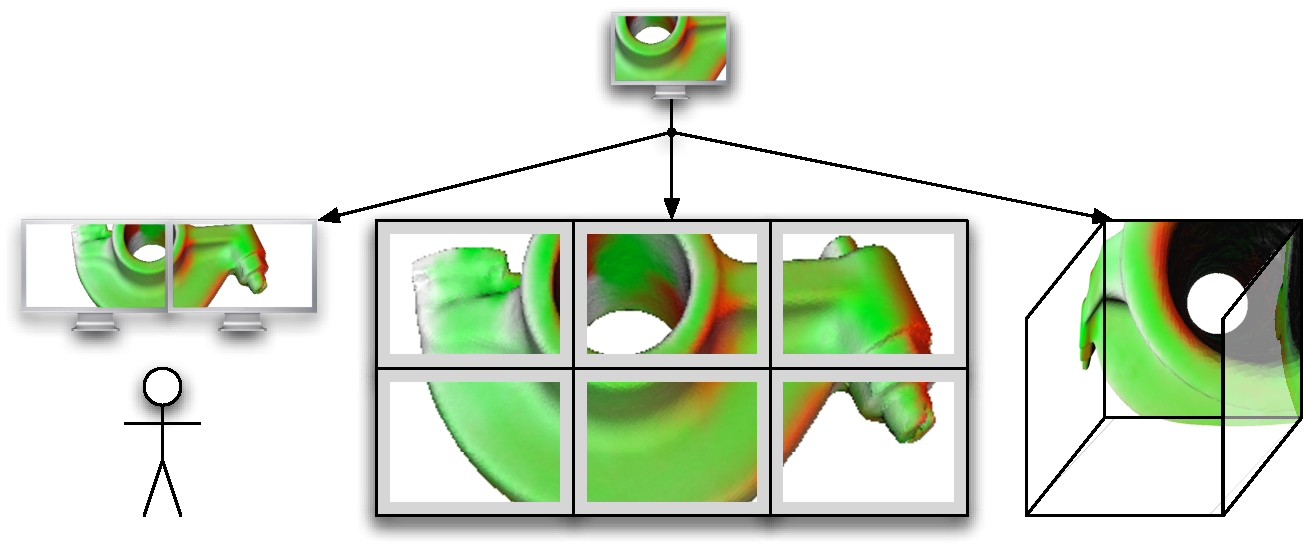
\includegraphics[width=0.9\columnwidth]{images/sp_to_mp.pdf}
%\caption{Some advanced display systems}
%\label{FIG_parallel}
%\end{figure}

\bibliographystyle{abbrvurl}
\bibliography{paper}
\end{document}
